\documentclass{gescons}

\genre {Entrevista}
\author{Fátima Fernandes}
\title{Imobilidade Física Vígil: Autopesquisa Experimentológica}


\begin{document}
    \makeentrevistatitle
    \coverart{back/Fatima_Fernandes}

    \begin{multicols}{2}

\begin{center}
    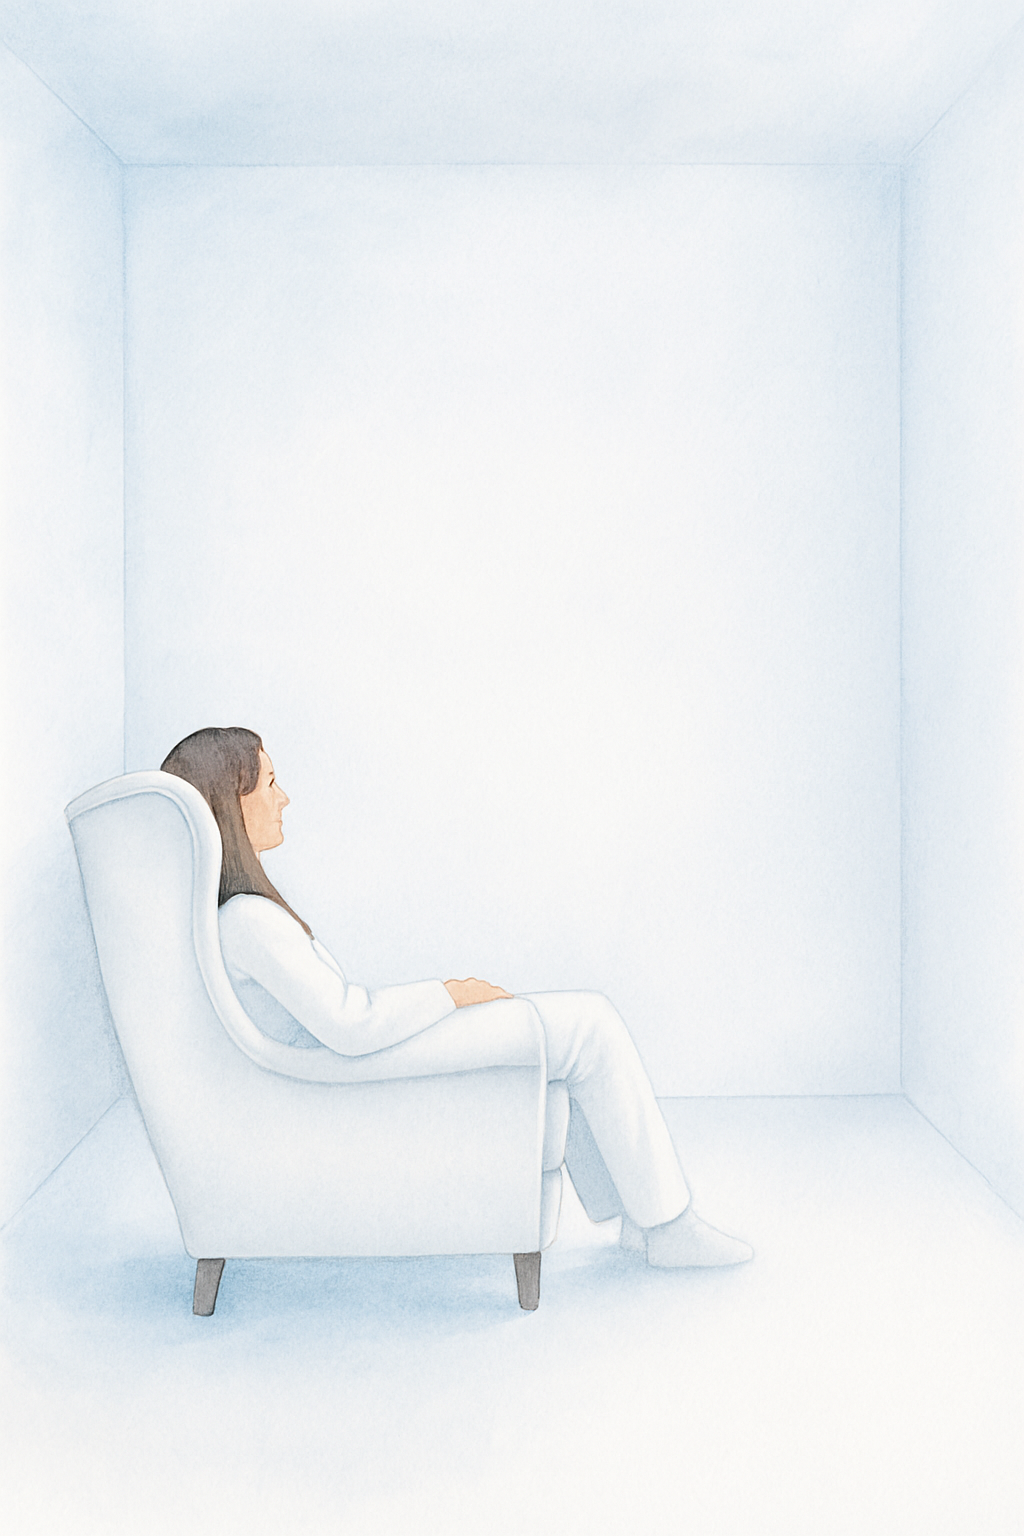
\includegraphics[width=6cm]{articles/entrevista/mockups/Fatima_Fernandes.png}
\end{center}


\textbf{1. Qual foi a motivação para a escrita da obra? Por que a definição deste tema para publicação de um livro?}

Utilizei a IFV como ferramenta de autopesquisa e também para melhorar o domínio da minha psicomotricidade. Sempre tive inspirações de amparadores ``desacelera''.

Depois de tantas experiências significativas me acionou o sentimento da retribuição. Escrever livro para contar um pouco da experiência. O nome do livro \emph{Imobilidade Física Vígil: Autopesquisa Experimentológica} encaixou muito bem para expor tais experiências.


\textbf{2. Quais foram as principais percepções, intra e extrafísicas, durante a pesquisa e a escrita da obra? E posterior ao lançamento?}

Durante a escrita o que mais ficou claro para mim é que determinadas recins são imprescindíveis para escrita do livro. Não basta ter experiência a escrita científica conscienciológica exige determinados requisitos que se o autor não atender a obra não sai. Fiz recins significativas de posturas religiosas para conseguir escrever as experiências de maneira técnica e científica.

\begin{pullquote}
``O  que mais ficou claro para mim é que determinadas recins são imprescindíveis para escrita do livro.''
\end{pullquote}

Um ponto que me chamou a atenção, quando o livro estava em processo de revisão, foi em várias situações recebia a inspiração sobre determinada frase e o local exato que estava escrita para ser revidada.

Tive várias projeções lúcidas sobre o andamento do livro durante o processo de revisão, diagramação até a impressão. Parece que o autor acompanha o processo de materialização da sua obra.

Posterior ao lançamento, percebi atendimento a grupo de consciexes ideológicas zombeteiras, conflito com o paradigma consciencial e inflexíveis a autoexperimentação.

\begin{pullquote}
``A IFV favorece a retilinearidade pensênica e a vontade autodeterminada, atributos imprescindíveis à escrita do livro.''
\end{pullquote}

A IFV favorece a retilinearidade pensênica e a vontade autodeterminada, atributos imprescindíveis à escrita do livro. Em tese os mais de 100 experimentos realizados por mim surtiram efeitos. Obra concluída!

O sentimento de satisfação de conclusão do livro conscienciológico é inexplicável. Tarefa cumprida!

\textbf{3. Qual o maior aprendizado com a escrita desta obra?}

O maior beneficiário da obra é o próprio autor.

\emph{O livro é um retrato expandido do autor para quem tem olhos de se autoavaliar.}


\textbf{4. O que poderia dizer como incentivo para que mais pesquisadores invistam na publicação de obras conscienciológicas?}

A CCCI e a UNIESCON oferecem inúmeras ferramentas, cursos, assessorias, para os neoautores e autores.

Resumo: ampliação da fundamentação cognitiva do paradigma consciencial.

A escrita da obra é teste teático mensurável do nível de entendimento do paradigma consciencial.


    
    \end{multicols}
\end{document}
